\documentclass[preview]{standalone}

\usepackage{amsmath}
\usepackage{amssymb}
\usepackage{stellar}
\usepackage{definitions}
\usepackage{bettelini}
\usepackage{tikz}
\usepackage{fancybox}
\usepackage{floatrow}
\usepackage{array}
\usepackage{makecell}

\usetikzlibrary{cd}

\begin{document}

\id{geoeconomica-cortina-ferro}
\genpage

\section{Cortina di ferro}

\plain{A fine della Seconda guerra mondiale, l'Europa si divise in due:}

\begin{snippet}{usa-vs-urss-illustration}
    \begin{center}
        %\figbox{
        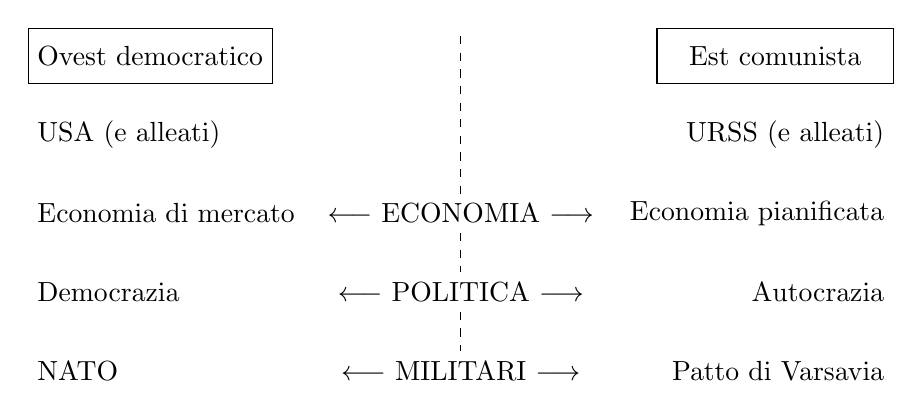
\begin{tikzpicture}
            \node[draw, minimum width=3cm, minimum height=0.7cm, anchor=west] at (0,0) {Ovest democratico};
            \node[anchor=west] at (0,-1) {USA (e alleati)};
            \node[anchor=west] at (0,-2) {Economia di mercato};
            \node[anchor=west] at (0,-3) {Democrazia};
            \node[anchor=west] at (0,-4) {NATO};
        
            \node[draw, minimum width=3cm, minimum height=0.7cm, anchor=east] at (11,0) {Est comunista};
            \node[anchor=east] at (11,-1) {URSS (e alleati)};
            \node[anchor=east] at (11,-2) {Economia pianificata};
            \node[anchor=east] at (11,-3) {Autocrazia};
            \node[anchor=east] at (11,-4) {Patto di Varsavia};
        
            \draw[dashed] (5.5,0.25) --  (5.5,-1.75);
            \draw[dashed] (5.5,-2.25) -- (5.5,-2.75);
            \draw[dashed] (5.5,-3.25) -- (5.5,-3.75);
        
            \node at (5.5,-2) {$\longleftarrow$\ ECONOMIA\ $\longrightarrow$};
            \node at (5.5,-3) {$\longleftarrow$\ POLITICA\ $\longrightarrow$};
            \node at (5.5,-4) {$\longleftarrow$\ MILITARI\ $\longrightarrow$};
        \end{tikzpicture}
        %}
    \end{center}
    \phantom{}
\end{snippet}

\begin{snippet}{cortina-di-ferro-expl}
    La Cortina di ferro era rappresentata economicamente, politicamente e ideologicamente e fisicamente da barriere
    di eserciti militari. Le suddivisioni delle due superpotenze mondiali postbelliche portò a un'escalation di un loro
    sviluppo forzato e all'inizio della Guerra fredda.
    \\
    L'Europa orientale, sotto influenza sovietica, si isolò e interruppe le comunicazioni e i commerci con l'occidente.
    \\
    Il simbolo della Cortina di ferro fu la Germania, in particolare con Berlino, il quale venne letteralmente diviso
    in due da un muro rinforzato militarmente.
\end{snippet}

% espandere commercio internazinoale
% regole vincolanti
% sistema stabile dei cambi
% 3 organi internazinoali: banca mondiale, FMI, GATT (-> WTF 1995)

\end{document}